% 学習結果説明（用語集と図の見方）
% results フォルダで「lualatex 学習結果説明.tex」を2回実行すると PDF を作り直せる（TeX Live の LuaLaTeX を使用）。
% 図は results/step2/ と results/step2_mcmc/ の PNG を相対パスで読み込む。
\documentclass[paper=a4paper,fontsize=10.5pt,line_length=44zw,number_of_lines=38]{jlreq}
\usepackage[haranoaji]{luatexja-preset}
\usepackage{amsmath}
\usepackage{graphicx}
\usepackage{booktabs}
\usepackage{tabularx}
\usepackage{enumitem}
\usepackage{float}
\usepackage{xcolor}
\usepackage[hidelinks,bookmarksnumbered]{hyperref}
\graphicspath{{step2/}{step2_mcmc/}}

\newcommand{\file}[1]{\texttt{\detokenize{#1}}}
\newcommand{\gd}{\dot{\gamma}}
% 用語集：「・用語：説明文」
\newenvironment{termlist}{\begin{itemize}[label=・,leftmargin=1\zw,labelwidth=1\zw,labelsep=0pt,itemsep=0.4ex,topsep=0.6ex,parsep=0pt]}{\end{itemize}}
\newcommand{\term}[1]{\item \textbf{#1}：}
% 図の見方の項目
\newenvironment{points}{\begin{itemize}[label=$\triangleright$,leftmargin=1.5\zw,itemsep=0.3ex,topsep=0.5ex,parsep=0pt]}{\end{itemize}}
\newcommand{\pt}[1]{\item \textbf{#1}：}
\renewcommand{\arraystretch}{1.25}

\title{樹脂粘度モデル開発　手順2の学習結果の説明\\[0.6ex]{\large 用語集とグラフの見方（機械学習・統計を初めて学ぶ人向け）}}
\author{}
\date{2026年10月6日}

\begin{document}
\maketitle
\tableofcontents

% =====================================================================
\section{この文書について}

この文書は、\file{results} フォルダにある手順2の学習結果（図と表）を、機械学習や統計を初めて学ぶ人でも読めるように説明したものです。射出成形と樹脂の粘度の基本は知っていることを前提にしています。

\begin{points}
\pt{対象の結果}次の2つのフォルダです。
  \begin{itemize}[leftmargin=1.5\zw,itemsep=0pt,topsep=0.2ex]
  \item \file{results/step2/}：手順2。ガウス過程回帰のハイパーパラメータを最尤推定で求めた結果（図4枚、表5つ）。
  \item \file{results/step2_mcmc/}：手順2の MCMC 版。ハイパーパラメータを MCMC で推定した結果（図7枚、表8つ）。
  \end{itemize}
\pt{読み方}2章で全体の流れをつかみ、分からない言葉は3章の用語集で調べてください。4章で図の見方、5章で表の見方、6章で結果のまとめを説明します。
\pt{数値について}文中の数値は、この文書を作った時点の results のファイルとノートの出力から取り出したものです。
\pt{元のノート}\file{01_機械学習コードフォルダ} の \file{手順2_現行モデル再現とリーク確認.ipynb} と \file{手順2_MCMC版_現行モデル再現とリーク確認.ipynb} です。
\pt{作り直し方}\file{results} フォルダで \texttt{lualatex 学習結果説明.tex} を2回実行すると、この PDF を作り直せます。
\end{points}

% =====================================================================
\section{何をしたか（概要）}

\subsection{目的}
射出成形の充填工程で測った「見かけの粘度」を成形条件から予測するモデルを、ガウス過程回帰（GPR）で作ろうとしています。手順2では、これまで使ってきた GPR（現行モデル）を同じ条件で作り直し、次の2点を確かめました。
\begin{enumerate}[itemsep=0.2ex,topsep=0.5ex]
\item 現行モデルが入力に使っている樹脂圧力 $P$ が、答えである粘度の計算式に含まれていないか（リーク）。
\item 学習データとテストデータの分け方によって、評価がどれだけ変わるか。
\end{enumerate}
MCMC 版では、ハイパーパラメータの決め方だけを変えて、同じことを確かめました。

\subsection{データ}
\file{学習データ6月発表時.csv} を使いました。
\begin{points}
\item 1,290 行（129 条件 $\times$ 各 10 ショット）です。1行が1ショットです。
\item 条件は、加熱シリンダ設定温度 190・210・230 ℃、キャビティ厚み 0.5・1.0・1.5・2.0 mm、射出率 12 水準（1.593〜169.92 cm$^3$/s）の組み合わせです。薄肉の低速など、成形できない組み合わせは含みません。
\item 各行には、見かけの粘度 $\eta$、見かけのせん断速度 $\gd$、流動先端温度 $T$、樹脂圧力 $P$ などの値が入っています。
\end{points}

\subsection{比べたモデルとデータの分け方}
4つのモデルと2つの分け方を組み合わせて比べました。目的変数（予測したい量）は、どのモデルも粘度の自然対数 $\ln\eta$ です。

\begin{table}[H]
\caption{比べた4つのモデル}
\begin{tabularx}{\linewidth}{@{}l>{\raggedright\arraybackslash}p{9\zw}X@{}}
\toprule
記号 & モデルと入力 & 意味 \\
\midrule
M1 & 現行の GPR\newline 入力：$\ln T$，$\ln P$，$\ln\gd$ & これまでのモデルを再現したもの。 \\
M2 & 線形回帰\newline 入力：$\ln P$，$\ln\gd$ & $P$ と $\gd$ だけの単純な式で、どこまで当たるかを見る。 \\
M3 & 線形回帰（算出式どおり）\newline 入力：$\ln(P-P_2)$，$\ln\gd$，$\ln H$ & 粘度を計算した式そのもの。これで完全に当たれば、粘度は $P$ から計算されている。 \\
M4 & $P$ を外した GPR\newline 入力：$\ln T$，$\ln\gd$ & $P$ がなくても予測できるかを見る。 \\
\bottomrule
\end{tabularx}
\end{table}

\begin{table}[H]
\caption{学習データとテストデータの分け方}
\begin{tabularx}{\linewidth}{@{}lX@{}}
\toprule
記号 & 分け方 \\
\midrule
S1 & せん断速度が 500〜1000 1/s の 90 行（9 条件）をテストデータにし、残りの 1,200 行で学習する。現行ノートと同じ分け方。同じ条件のショットが学習とテストに分かれることはない。 \\
S2 & ランダムに選んだ2割（258 行）をテストデータにし、残りの 1,032 行で学習する。テストを含む 113 条件のすべてで、同じ条件の別のショットが学習データにも入っている。 \\
\bottomrule
\end{tabularx}
\end{table}

\subsection{ハイパーパラメータの求め方}
\begin{points}
\pt{手順2（最尤推定）}対数周辺尤度が最も大きくなる値を、1組だけ求めました。
\pt{MCMC 版}もっともらしい値の分布を、たくさんのサンプルで表しました。自作の適応型メトロポリス法を使い、4本のチェーンで、調整 3,000 回のあと本番を 8,000 回（S2・M1 だけ 20,000 回）行いました。
\end{points}

% =====================================================================
\section{用語集}

「・用語：説明」の形で、分野ごとに並べました。$\eta$ や $\gd$ などの記号は、図の中でも使っています。

\subsection{粘度と測定に関する用語}
\begin{termlist}
\term{見かけの粘度 $\eta$ [Pa$\cdot$s]}樹脂の流れにくさ。ここでは、キャビティの中の2点の圧力センサの値から計算した値です。せん断発熱や冷却の影響も含んだ「見かけ」の値として扱います。
\term{見かけのせん断速度 $\gd$ [1/s]}流れの中で、樹脂がずれるように変形する速さ。射出率が大きいほど大きくなります。樹脂の粘度は、$\gd$ が大きいほど下がります（せん断流動化）。
\term{見かけの壁面せん断応力 $\tau$ [Pa]}流れが壁面を引きずる力の強さ。$\tau = \eta \times \gd$ の関係があります。
\term{圧力損失 $\Delta P$ [Pa]}2つのセンサの間で失われた圧力。粘度の計算に使います。今回のデータでは $\Delta P = P - P_2$ です。
\term{樹脂圧力 $P$ と $P_2$}$P$ は、2点目のセンサに樹脂が届いたときの1点目の圧力です（CSV の「流動中樹脂圧力P」）。$P_2$ はそのときの2点目の圧力で、データから約 0.400 MPa と求まりました。
\term{センサ間距離 $L$}2つの圧力センサの距離。データから約 17.50 mm と求まりました。
\term{キャビティ厚み $H$ [mm]}平板のキャビティの厚み。0.5・1.0・1.5・2.0 mm の4水準です。
\term{射出率 [cm$^3$/s]}1秒あたりに押し出す樹脂の体積（成形機の設定値）。
\term{加熱シリンダ設定温度（設定温度）}成形機に設定した樹脂の温度。190・210・230 ℃ の3水準です。CSV の元ファイル名から取り出しました。
\term{流動先端温度 $T$}センサの間を流れている樹脂の先端の温度（実測値）。流れの速さによって上下するので、流れの「結果」でもあります。
\term{条件とショット}条件は、設定温度・厚み・射出率の組み合わせです（129 通り）。各条件で 10 回成形しており、1回の成形をショットと呼びます。
\term{$\ln$ と $\log_{10}$}$\ln$ は自然対数（$e \approx 2.718$ を底とする対数）、$\log_{10}$ は常用対数（10 を底とする対数）です。粘度は桁で変わるので、計算は対数で行います。$\ln\eta$ の差 0.1 は、粘度の約 1.1 倍の違いに当たります。
\end{termlist}

\subsection{データの扱いに関する用語}
\begin{termlist}
\term{目的変数}予測したい量。ここでは $\ln\eta$（粘度の自然対数）です。
\term{説明変数（入力）}予測の手がかりにする量。モデルごとに違います（2章の表1）。
\term{学習データ}モデルを作るとき（モデルの中の値を決めるとき）に使うデータ。
\term{テストデータ}学習には使わず、できたモデルの予測がどれだけ当たるかを確かめるためだけに使うデータ。実際に予測したい「まだ測っていないデータ」の代わりです。
\term{データの分割}全データを、学習データとテストデータに分けること。分け方によって、評価の厳しさが変わります。
\term{条件単位の分割}同じ条件の 10 ショットを、学習とテストのどちらか一方にまとめて入れる分け方。S1 はこれに当たります。ランダムに分けると（S2）、同じ条件のショットが学習とテストの両方に入り、「ほとんど同じデータでの答え合わせ」になって、評価が甘くなります。
\term{標準化}入力の値から平均を引き、標準偏差で割って、平均 0・ばらつき 1 にそろえること。単位や大きさの違う入力を、公平に扱うためです。
\term{中心化}値から平均を引いて、平均を 0 にそろえること。ここでは $\ln\eta$ を中心化してから GPR に入れています。
\term{リーク（目的変数のリーク）}答え（目的変数）を計算するのに使った値が入力に紛れ込み、モデルが答えを「計算」できてしまうこと。精度は高く見えますが、実際に予測したい場面ではその入力を先に知ることができないので、役に立ちません。今回は樹脂圧力 $P$ がこれに当たります。
\term{内挿と外挿}学習データの範囲の内側を予測するのが内挿、外側を予測するのが外挿です。一般に外挿のほうが難しくなります。
\end{termlist}

\subsection{モデルに関する用語}
\begin{termlist}
\term{回帰}入力から数値（ここでは粘度）を予測すること。また、そのための式やモデル。
\term{線形回帰}入力に重みを掛けて足し合わせ、定数を加えた式で予測する、最も単純な回帰。重みは最小二乗法で決めます。
\term{最小二乗法}予測と実測の差を2乗して合計した値が最も小さくなるように、式の係数を決める方法。
\term{ガウス過程回帰（GPR）}「似た入力には似た出力が対応する」という考えに基づいて、データの間を滑らかにつなぐ回帰の方法。予測値と一緒に、予測のばらつき（不確かさ）も出せるのが特長です。近くにデータが少ない所では、ばらつきが大きくなります。
\term{カーネル（共分散関数）}2つの入力がどれくらい「似ているか」を決める関数。GPR の性質（滑らかさなど）はカーネルで決まります。
\term{Matern 5/2 カーネル}よく使われるカーネルの一つ。入力どうしの距離が近いほど似ているとみなし、ほどよく滑らかな関数を表せます。現行モデルで使っています。
\term{ARD（関連度の自動決定）}入力ごとに別々の長さスケールを持たせる仕組み。長さスケールを見れば、どの入力がよく効いているかが分かります。
\term{長さスケール}入力がどれくらい変わると出力が大きく変わるかを表す目安（ここでは標準化した入力に対する値）。小さいほどその入力の変化に敏感で、よく効いていることを表します。大きいほど効き方がゆるやかです。
\term{振幅}GPR が表す関数の大きさ（目的変数がどれくらいの幅で変わり得るか）の目安。カーネルの中では振幅の2乗（振幅$^2$）を使います。
\term{ノイズ分散}同じ条件でもショットごとにばらつく大きさ（成形や測定のばらつき）を表す値。カーネルの「ホワイトノイズ」の部分です。今回は $\ln\eta$ の分散で、探索範囲の下限 0.001（標準偏差で約 0.032、粘度で約 3\%）に張り付きました。
\term{ハイパーパラメータ}モデルの形を決める設定値。GPR では、振幅・長さスケール・ノイズ分散です。データから推定します。
\term{探索範囲}ハイパーパラメータが取り得る範囲。現行コードでは、振幅$^2$ が 0.001〜1000、長さスケールが 0.01〜100、ノイズ分散が 0.001〜10 です。
\end{termlist}

\subsection{推定に関する用語}
\begin{termlist}
\term{対数周辺尤度}あるハイパーパラメータの値のもとで、学習データがどれくらい「もっともらしく」得られるかを表す数（の対数）。大きいほど、データによく合っています。
\term{最尤推定}対数周辺尤度が最も大きくなるハイパーパラメータを、1組だけ選ぶ方法。手順2はこれです。
\term{ベイズ推定}値を1つに決めずに、「どの値がどれくらいありそうか」を確率の分布で表す推定の方法。
\term{事前分布}データを見る前に、ハイパーパラメータの値をどう考えるかを表す分布。今回は、探索範囲の中で、対数の目盛りの上で一様（どの値も同じくらいありそう）としました。
\term{事後分布}データを見たあとの、ハイパーパラメータの値のもっともらしさの分布。今回は、探索範囲の中で exp(対数周辺尤度) に比例するので、山の頂上（最頻値）は最尤推定の値と一致します。
\term{MCMC（マルコフ連鎖モンテカルロ法）}事後分布を直接計算する代わりに、分布に従う「サンプル」をたくさん集めて分布を表す方法。サンプルの平均や広がりから、値の目安と不確かさが分かります。
\term{メトロポリス法}MCMC の基本的な方法。今いる値の近くに次の候補をランダムに出し、候補のほうがもっともらしければ移動し、そうでなければ確率的に移動するか、その場にとどまります。これを繰り返します。
\term{提案分布}次の候補を出すときに使う分布。候補を、どの方向に、どれくらいの距離に出すかを決めます。
\term{採択率}候補が受け入れられた（移動した）割合。大きすぎても小さすぎても効率が悪く、0.2〜0.3 程度がよいとされます。今回は 0.20〜0.27 でした。
\term{適応型}調整期間に、それまでのサンプルから分布の広がりや向き（パラメータどうしの相関）を学び、提案分布を自動で合わせること。
\term{調整期間と本番}調整期間（今回 3,000 回）は、出発点から分布の山に近づき、提案分布を合わせるための期間で、そのサンプルは捨てます。本番（8,000 回。S2・M1 だけ 20,000 回）は提案分布を固定して歩き、そのサンプルを結果に使います。
\term{チェーン}MCMC の一続きのサンプル。別々の出発点から複数本（今回 4 本）走らせ、結果がそろうかどうかで信頼性を確かめます。
\term{予測分布}ある入力に対する予測値の分布。GPR では、平均（予測値）と標準偏差（ばらつき）で表される正規分布です。
\term{混合分布}複数の分布を混ぜ合わせた分布。MCMC 版では、事後分布から選んだ 200 組のハイパーパラメータのそれぞれで予測分布を求め、それらを同じ重みで混ぜたものを予測分布にしました。こうすると、ハイパーパラメータの不確かさも予測のばらつきに含まれます。
\term{信用区間}事後分布の中で、値が入る確率が 95\% などになる範囲。この文書では、2.5\% 点から 97.5\% 点までの範囲です。
\term{予測区間}新しく測ったときの値が、95\% などの確率で入る範囲。ショットごとのばらつき（ノイズ）も含みます。
\end{termlist}

\subsection{収束の確認に関する用語}
\begin{termlist}
\term{収束}MCMC のサンプルが、目標の分布をきちんと表すようになった状態。チェーンが十分に長くないと、分布の一部しか表せていないことがあります。
\term{R-hat（アールハット）}複数のチェーンの結果がそろっているかを表す指標。1 に近いほどよく、1.01 以下が目安です。チェーンごとに違う所を歩いていると、1 より大きくなります。
\term{有効サンプル数（ESS）}続くサンプルどうしは似ているので、その重なりを差し引いて「互いに独立なサンプル何個分の情報があるか」に直した数。400 以上が目安です。bulk は分布の中心付近、tail は分布の裾（2.5\% 点や 97.5\% 点など）の精度に関わります。
\term{モンテカルロ誤差}サンプルの数が有限であることによる、平均などの計算の誤差。有効サンプル数の平方根に反比例して小さくなります。
\term{大数の法則と中心極限定理}サンプルを増やすと、平均は真の値に近づき（大数の法則）、その誤差は $1/\sqrt{\text{有効サンプル数}}$ に比例して小さくなります（中心極限定理）。MCMC で反復を増やすと R-hat や ESS が良くなるのはこのためです。これは計算の精度が上がるだけで、モデルや予測そのものは変わりません。
\end{termlist}

\subsection{評価の指標}
\begin{termlist}
\term{決定係数 $R^2$}予測が、データのばらつきをどれだけ説明できたかを表す指標。1 なら完全に一致、0 なら「いつも平均値を答える」のと同じ、マイナスならそれより悪いことを表します。この文書では、主に $\ln\eta$ で計算した値を示します。現行ノートは粘度そのもので計算しているので、値が少し違います（例：S1・M1 で、$\ln\eta$ では 0.9823、粘度そのものでは 0.9666）。また、テストデータの値の範囲が狭いと、同じ誤差でも $R^2$ は小さくなります。
\term{RMSE（二乗平均平方根誤差）}予測と実測の差の、平均的な大きさ。$\ln\eta$ の RMSE が 0.05 なら、粘度で約 5\% の誤差に当たります。小さいほどよい指標です。
\term{95\% 予測区間の被覆率}テストデータのうち、95\% 予測区間に実測値が入った割合。0.95 に近いのが理想です。小さすぎるとばらつきを小さく見積もりすぎ（自信過剰）、1.00 は区間が広すぎる可能性があります。
\term{NLPD（負の対数予測密度）}予測分布のもとで、実測値がどれくらい「ありそう」だったかを表す指標。予測値の当たり具合と、予測のばらつきの見積もりの適切さを、まとめて評価します。小さい（マイナスに大きい）ほどよい指標です。
\term{予測標準偏差の平均}テストデータでの予測のばらつき（$\ln\eta$ の標準偏差）の平均。予測区間の広さの目安です。
\end{termlist}

\subsection{図に関する用語}
\begin{termlist}
\term{パリティ図}横軸に実測値、縦軸に予測値をとって点を打った図。点が対角線（理想線）に乗るほど、予測が当たっています。
\term{理想線}パリティ図の対角線（予測値 = 実測値）。図では赤い破線です。
\term{誤差棒}点から上下に伸びる線。予測のばらつき（ここでは 95\% 予測区間）を表します。
\term{対数軸}目盛りが 1，10，100 のように、桁ごとに等間隔になる軸。桁で変わる量（粘度やせん断速度）を見やすくします。両方の軸が対数軸の図で直線に見える関係は、べき乗の関係を表します。
\term{ヒストグラム}値をいくつかの区間に分け、それぞれの区間に入るサンプルの数（または割合）を棒で表した図。分布の形が分かります。
\term{トレース図}MCMC のサンプルの値を、反復の順に線でつないだ図。チェーンがよく混ざっているかを見ます。
\term{帯}予測曲線の周りの薄い色の範囲。予測の 95\% 区間を表します。
\end{termlist}

% =====================================================================
\section{図の見方}

図ごとに、「何を示す図か」「軸と記号」「見るポイント」「今回の結果」の順に説明します。図のファイルは \file{results} の下にあります。

% ---------------------------------------------------------------------
\subsection{図1：粘度の算出式の確認}
\begin{figure}[H]
\centering
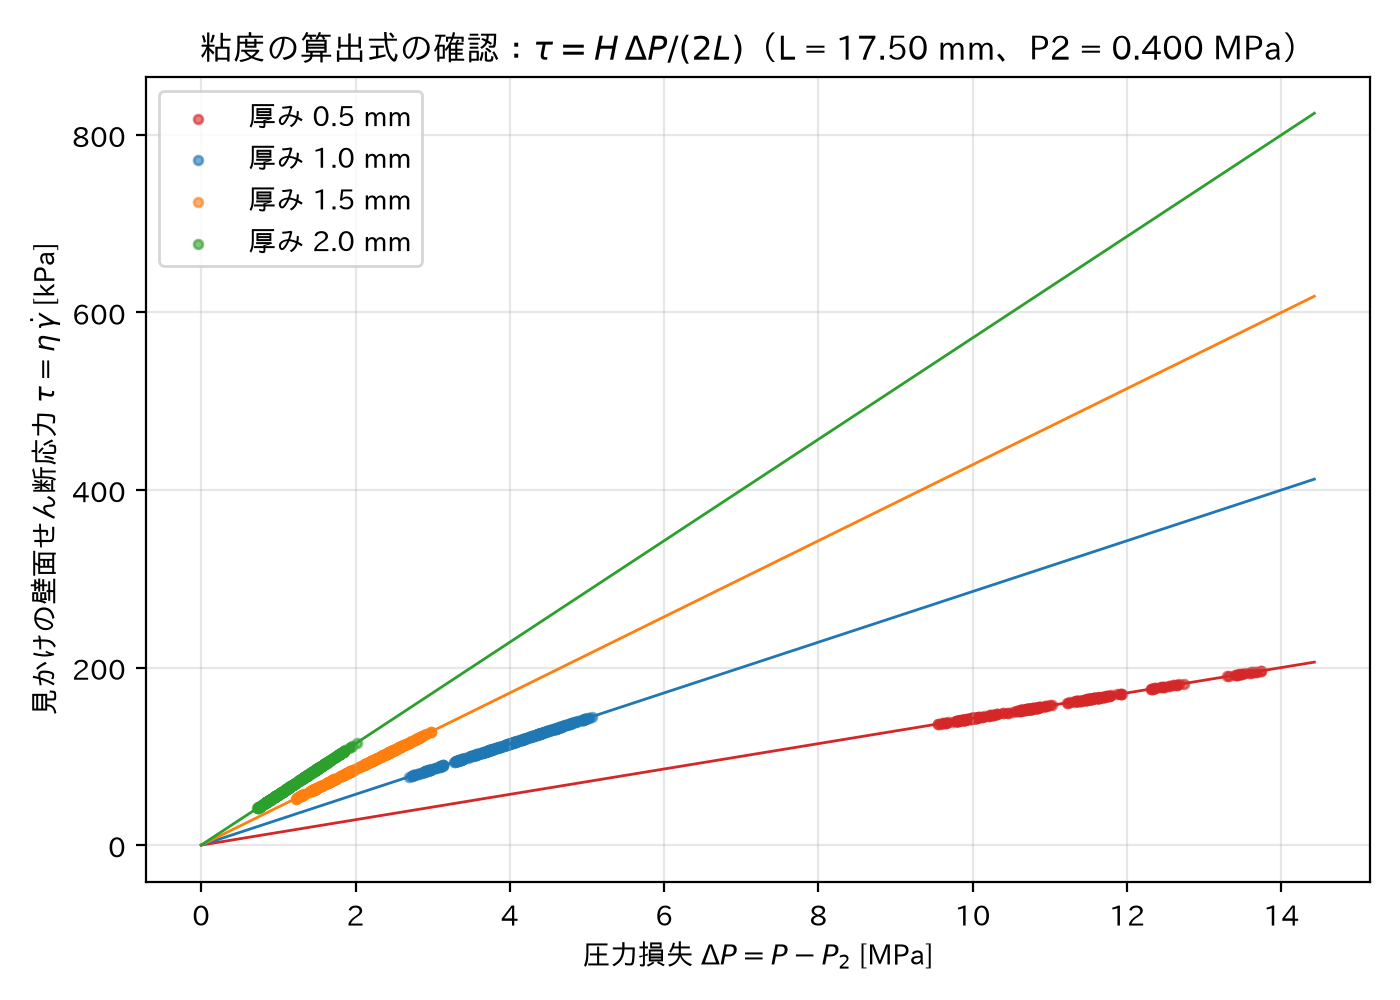
\includegraphics[width=0.74\linewidth]{fig1_formula_check.png}
\caption{粘度の算出式の確認}
\end{figure}
\begin{points}
\pt{ファイル}\file{results/step2/fig1_formula_check.png}
\pt{何を示す図か}CSV の粘度が、樹脂圧力 $P$ から計算された値かどうかを確かめる図です。
\pt{軸}横軸は圧力損失 $\Delta P = P - P_2$ [MPa]、縦軸は見かけの壁面せん断応力 $\tau = \eta \times \gd$ [kPa] です。
\pt{記号}点の1つが1ショットで、色はキャビティ厚みです。直線は、$\tau = H\,\Delta P/(2L)$ の式を厚みごとに引いたものです。
\pt{見るポイント}点が厚みごとの直線にぴったり乗っていれば、粘度はこの式で $P$ から計算されています。
\pt{今回の結果}全 1,290 ショットが直線に乗り、ずれは最大でも 0.035\% でした（$L$ = 17.50 mm、$P_2$ = 0.400 MPa）。$P$・$\gd$・厚みが分かれば、粘度は計算で決まります。つまり、$P$ を入力にするとリークになります。
\end{points}

% ---------------------------------------------------------------------
\subsection{図2：パリティ図}
\begin{figure}[H]
\centering
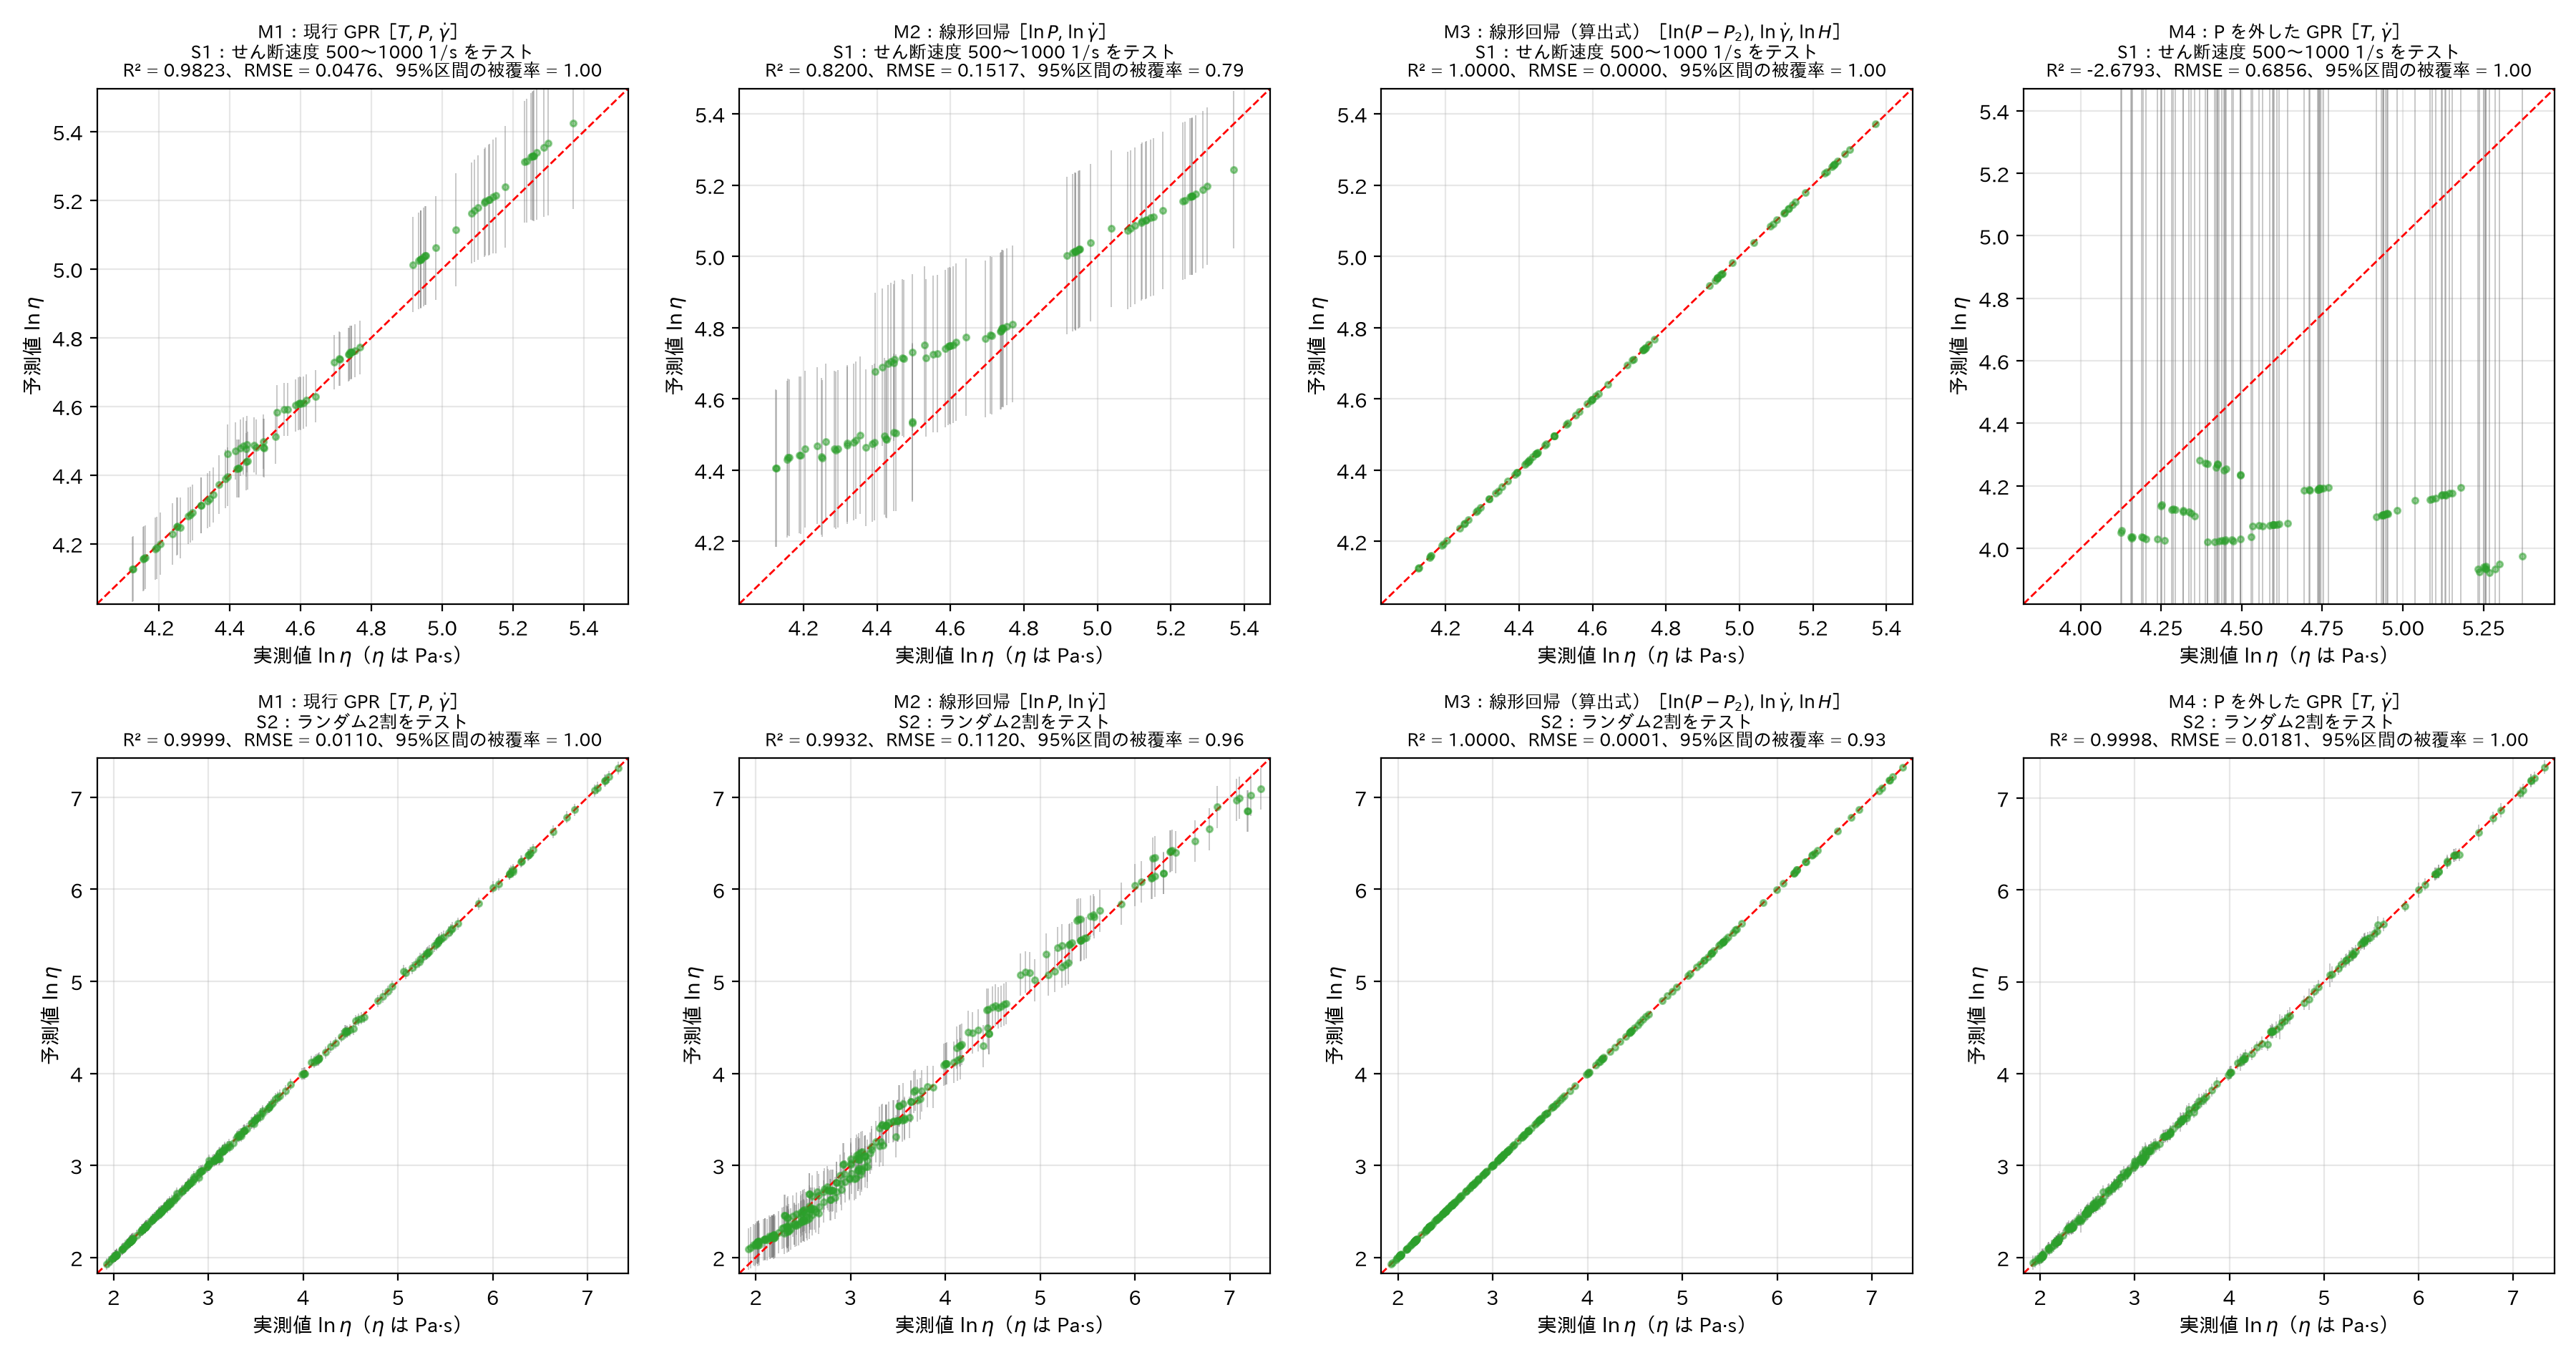
\includegraphics[width=\linewidth]{fig2_parity_ln_eta.png}
\caption{テストデータでのパリティ図（上段 S1、下段 S2。列は M1〜M4）}
\end{figure}
\begin{points}
\pt{ファイル}\file{results/step2/fig2_parity_ln_eta.png}
\pt{何を示す図か}4つのモデル（列）の予測が、テストデータでどれだけ当たったかを、2つの分け方（行）で比べる図です。
\pt{軸}横軸は実測の $\ln\eta$、縦軸は予測の $\ln\eta$ です。
\pt{記号}緑の点が1ショット、灰色の縦線が 95\% 予測区間、赤い破線が理想線です。各パネルの上に、モデル、分け方、$R^2$・RMSE・被覆率を示しました。
\pt{見るポイント}点が赤い破線に沿っているか。灰色の縦線が赤い破線にかかっているか（被覆率）。
\pt{今回の結果（上段 S1）}現行の M1 は $R^2$ = 0.9823 と高く、算出式どおりの M3 は 1.0000 で完全に当たりました。ところが、$P$ を外した M4 は $-2.68$ で、予測がほぼ平らになり、まったく当たりません。M4 の縦線がとても長いのは、モデルが「分からない」と示しているためです。現行モデルの高い精度は、$P$（リーク）によるものだと分かります。
\pt{今回の結果（下段 S2）}ランダムに分けると、$P$ を外した M4 でも $R^2$ = 0.9998 と高くなります。テストを含む 113 条件のすべてで、同じ条件の別のショットが学習データに入っているので、それを覚えて答えられてしまうためです。ランダムな分け方では評価が甘くなります。
\end{points}

\begin{table}[H]
\caption{テストデータでの指標（$\ln\eta$ で計算。\file{step2/metrics.csv}）}
\begin{tabularx}{\linewidth}{@{}X*{6}{r}@{}}
\toprule
 & \multicolumn{3}{c}{S1（せん断速度の帯）} & \multicolumn{3}{c}{S2（ランダム2割）} \\
\cmidrule(lr){2-4}\cmidrule(l){5-7}
モデル & $R^2$ & RMSE & 被覆率 & $R^2$ & RMSE & 被覆率 \\
\midrule
M1 現行 GPR & 0.982 & 0.048 & 1.00 & 1.000 & 0.011 & 1.00 \\
M2 線形回帰 & 0.820 & 0.152 & 0.79 & 0.993 & 0.112 & 0.96 \\
M3 線形回帰（算出式） & 1.000 & 0.000 & 1.00 & 1.000 & 0.000 & 0.93 \\
M4 P を外した GPR & $-2.679$ & 0.686 & 1.00 & 1.000 & 0.018 & 1.00 \\
\bottomrule
\end{tabularx}
\end{table}

% ---------------------------------------------------------------------
\subsection{図3：設定温度ごとのデータ}
\begin{figure}[H]
\centering
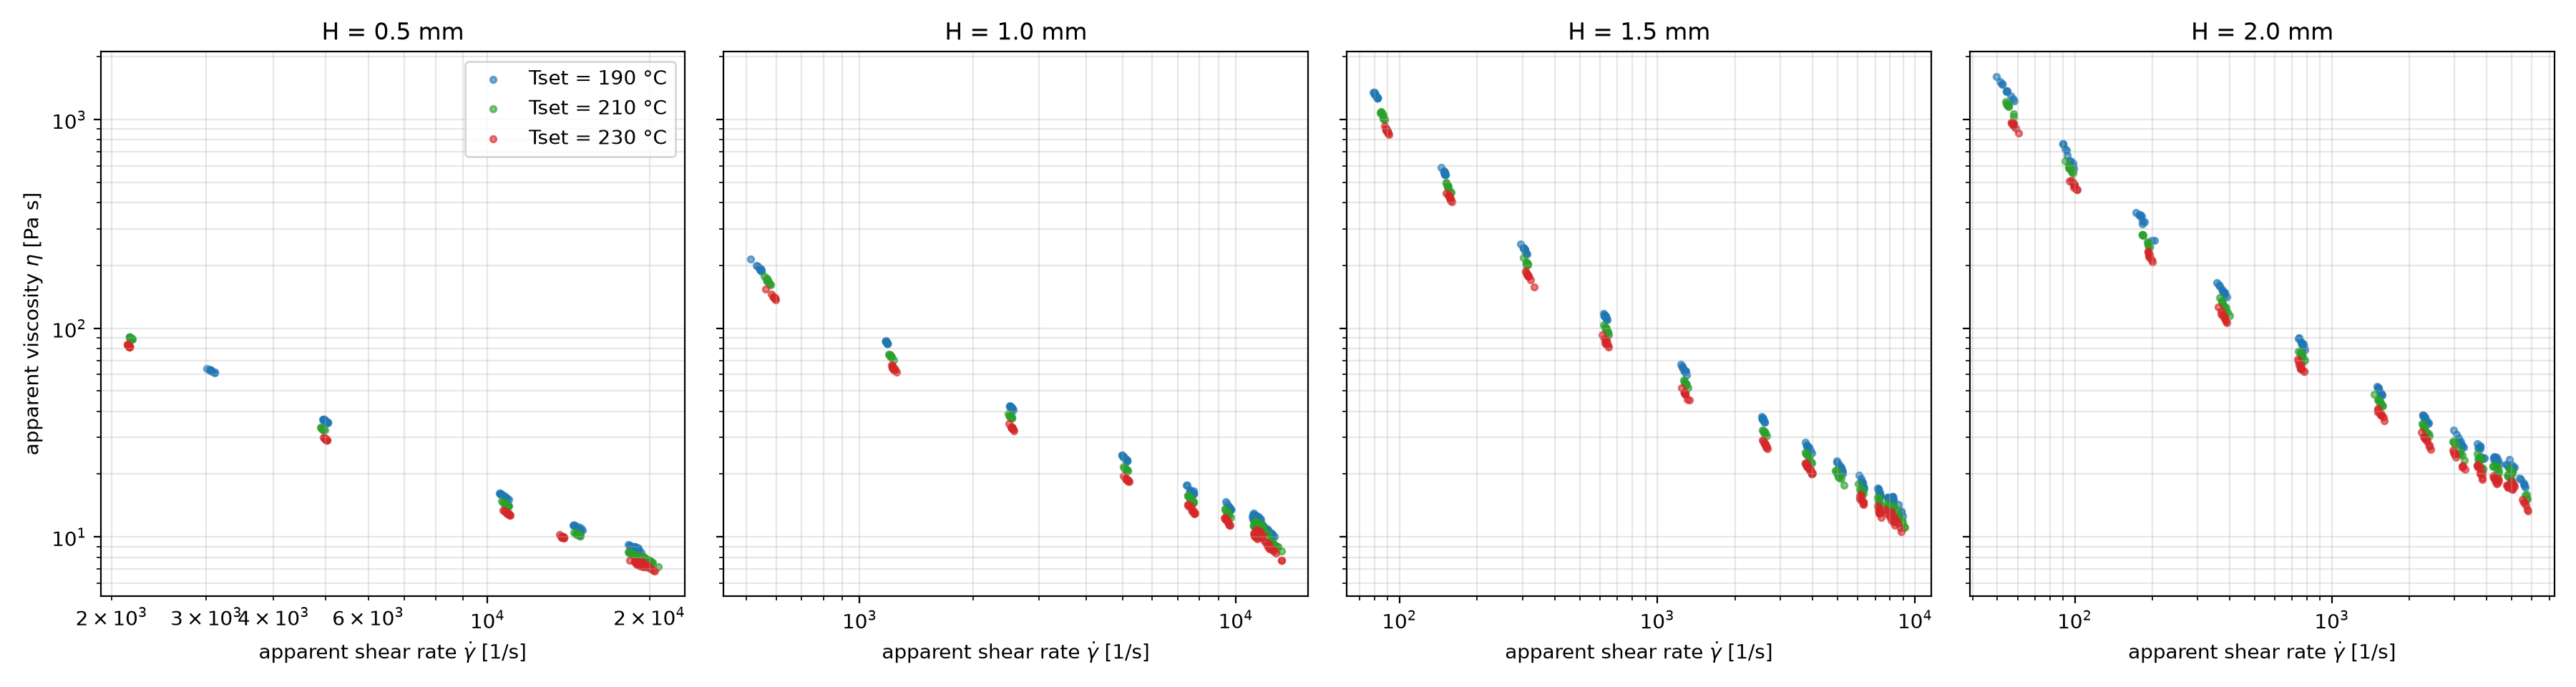
\includegraphics[width=\linewidth]{fig3_data_by_Tset.png}
\caption{厚みごと・設定温度ごとの粘度とせん断速度（データそのもの）}
\end{figure}
\begin{points}
\pt{ファイル}\file{results/step2/fig3_data_by_Tset.png}
\pt{何を示す図か}モデルの予測ではなく、データそのものです。厚みごと（パネル）に、粘度とせん断速度の関係を、設定温度で色分けしました。
\pt{軸}横軸は見かけのせん断速度 $\gd$ [1/s]、縦軸は見かけの粘度 $\eta$ [Pa$\cdot$s] で、どちらも対数軸です。
\pt{記号}点の1つが1ショットです。青・緑・赤が、設定温度 190・210・230 ℃ です。
\pt{見るポイント}同じせん断速度で、色によって高さ（粘度）が違うか。右下がりの傾き（せん断速度が上がると粘度が下がる）。
\pt{今回の結果}どの厚みでも、温度が低いほど粘度が高くなっています。同じ厚み・同じ射出率どうしで比べると、190 ℃ の粘度は 230 ℃ の約 1.24 倍（中央値）でした。温度の効果は、データにははっきり表れています。
\end{points}

% ---------------------------------------------------------------------
\subsection{図4：現行モデル M1 の予測曲線}
\begin{figure}[H]
\centering
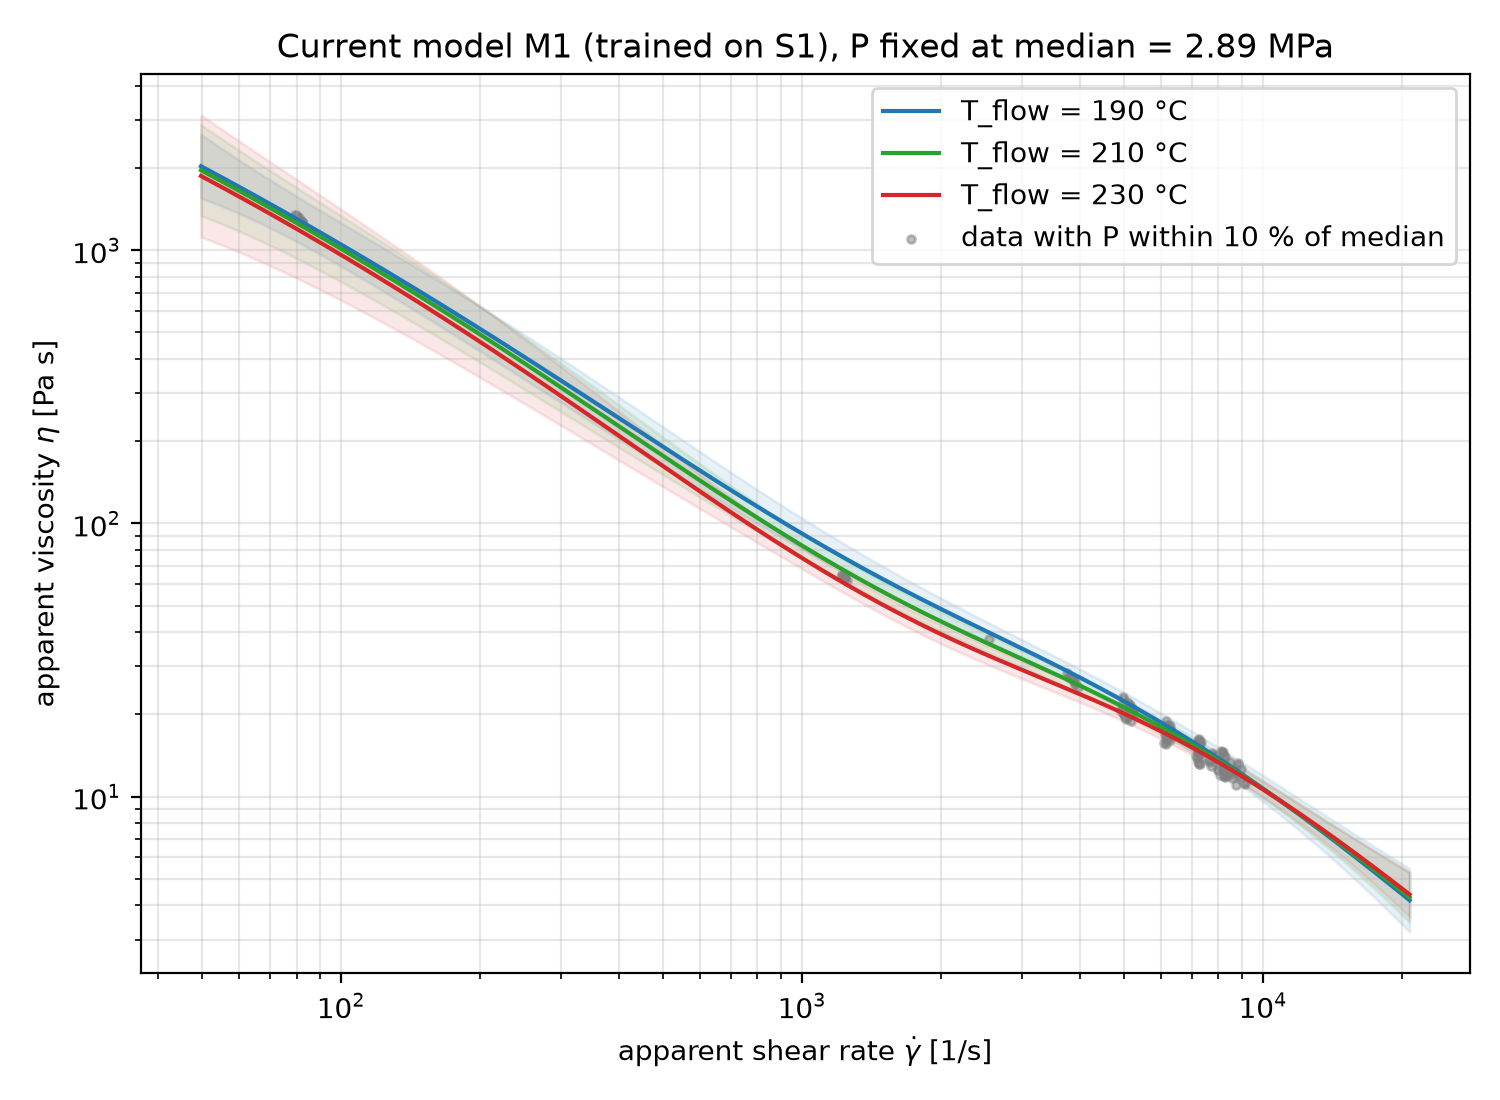
\includegraphics[width=0.74\linewidth]{fig4_M1_curves_by_T.png}
\caption{現行モデル M1 の予測曲線（$P$ を固定し、流動先端温度だけを変えたもの）}
\end{figure}
\begin{points}
\pt{ファイル}\file{results/step2/fig4_M1_curves_by_T.png}
\pt{何を示す図か}現行モデル M1（S1 で学習）で、$P$ を中央値（2.89 MPa）に固定し、流動先端温度だけを 190・210・230 ℃ に変えたときの予測です。
\pt{軸}横軸は $\gd$ [1/s]、縦軸は $\eta$ [Pa$\cdot$s] で、どちらも対数軸です。
\pt{記号}線が予測、薄い帯が 95\% 予測区間、灰色の点は $P$ が中央値の $\pm$10\% 以内のショットです。
\pt{見るポイント}温度を変えたときに、曲線がどれだけ動くか。曲線の傾き。
\pt{今回の結果}3本の曲線はほとんど重なりました（190 ℃ と 230 ℃ の差は平均で約 1.15 倍、最大でも 1.24 倍）。傾きは約 $-0.99$ で、これは「$P$（せん断応力）を一定にすると $\eta = \tau / \gd$ になる」という定義そのものです。$P$ を固定すると粘度はほぼ計算で決まってしまい、温度の効果は表に出てきません。図3のデータには温度の効果があるのに、現行モデルではそれが使われていないことが分かります。
\end{points}

% ---------------------------------------------------------------------
\subsection{図5〜8：トレース図}
\begin{figure}[H]
\centering
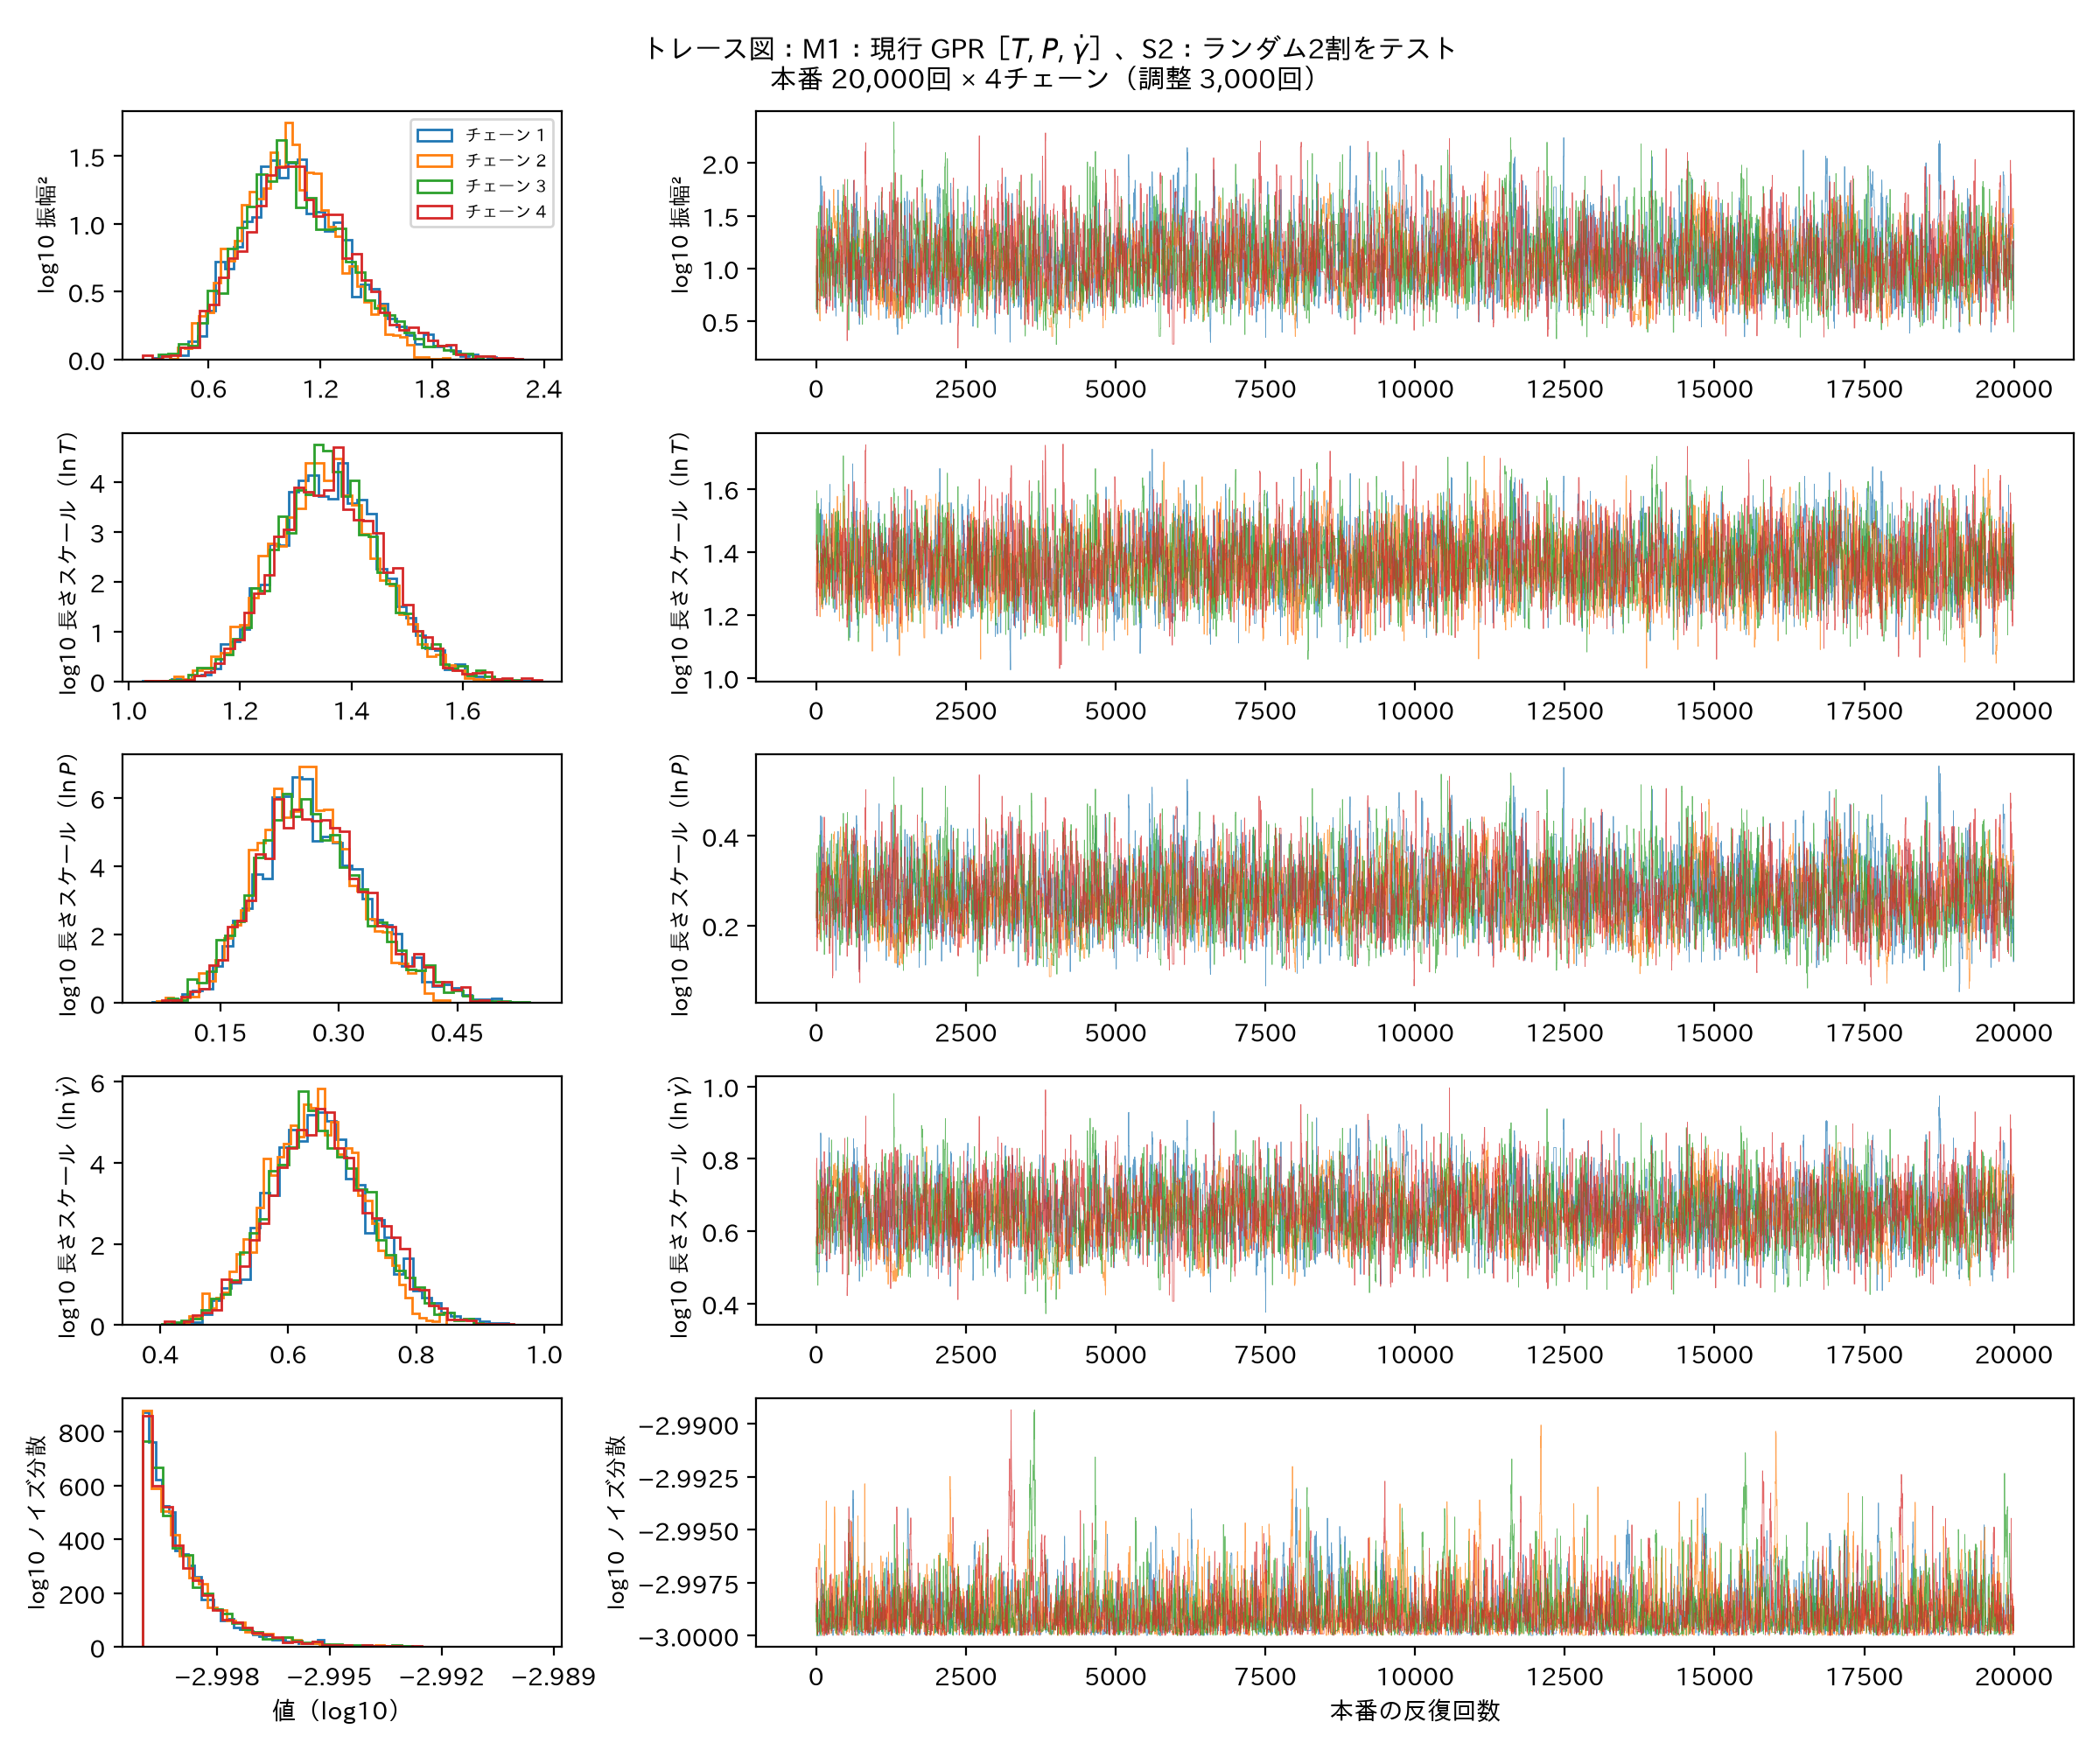
\includegraphics[width=0.86\linewidth]{fig_trace_S2_M1.png}
\caption{トレース図の例（S2・M1）}
\end{figure}
\begin{points}
\pt{ファイル}\file{results/step2_mcmc/fig_trace_*.png}
\pt{何を示す図か}MCMC のサンプルの様子です。1枚が1つの組み合わせ（分け方とモデル）で、行がハイパーパラメータ（振幅$^2$、長さスケール、ノイズ分散）です。ほかの3枚（\file{fig_trace_S1_M1.png}、\file{fig_trace_S1_M4.png}、\file{fig_trace_S2_M4.png}）も同じ見方です。
\pt{左の列}チェーンごとの分布（ヒストグラムの輪郭）です。横軸は値の $\log_{10}$ です。
\pt{右の列}本番の反復ごとの値の動きです。横軸は反復回数、縦軸は値の $\log_{10}$ で、色がチェーンです。
\pt{見るポイント}右の列で、4色の線が同じ範囲を細かく上下し、毛虫のように重なっているか（よく混ざっている）。1色だけ離れた所にいる、ゆっくり漂う、といった様子はよくありません。左の列で、4本の輪郭がほぼ重なるか（R-hat が 1 に近い）。
\pt{今回の結果}4枚とも、4本のチェーンがよく重なっています。全パラメータで R-hat は最大 1.004、有効サンプル数は最小 1,063 で、収束の目安（R-hat 1.01 以下、ESS 400 以上）を満たしました。ノイズ分散の分布が左端で切れた片寄った形をしているのは、探索範囲の下限（0.001。$\log_{10}$ で $-3$）に張り付いているためです。
\pt{S2・M1 だけ回数が多い理由}本番 8,000 回では R-hat が 1.012 で目安をわずかに超えたので、同じチェーンを 20,000 回まで延長しました。延長しても予測の指標はほとんど変わらず、計算の精度が上がっただけです。
\end{points}

\begin{table}[H]
\caption{組み合わせごとのサンプリングの回数と収束（\file{step2_mcmc/sampler_stats.csv}。4チェーン、調整 3,000 回）}
\begin{tabularx}{\linewidth}{@{}X*{5}{r}@{}}
\toprule
組み合わせ & 本番の回数 & 時間（分） & 採択率 & R-hat の最大 & ESS の最小 \\
\midrule
S1・M1 & 8,000 & 13.1 & 0.23〜0.27 & 1.003 & 1,063 \\
S1・M4 & 8,000 & 14.8 & 0.20〜0.24 & 1.003 & 1,174 \\
S2・M1 & 20,000 & 18.3 & 0.20〜0.25 & 1.004 & 1,116 \\
S2・M4 & 8,000 & 8.7 & 0.20〜0.25 & 1.004 & 1,229 \\
\bottomrule
\end{tabularx}
\end{table}

% ---------------------------------------------------------------------
\subsection{図9：事後分布と最尤推定値}
\begin{figure}[H]
\centering
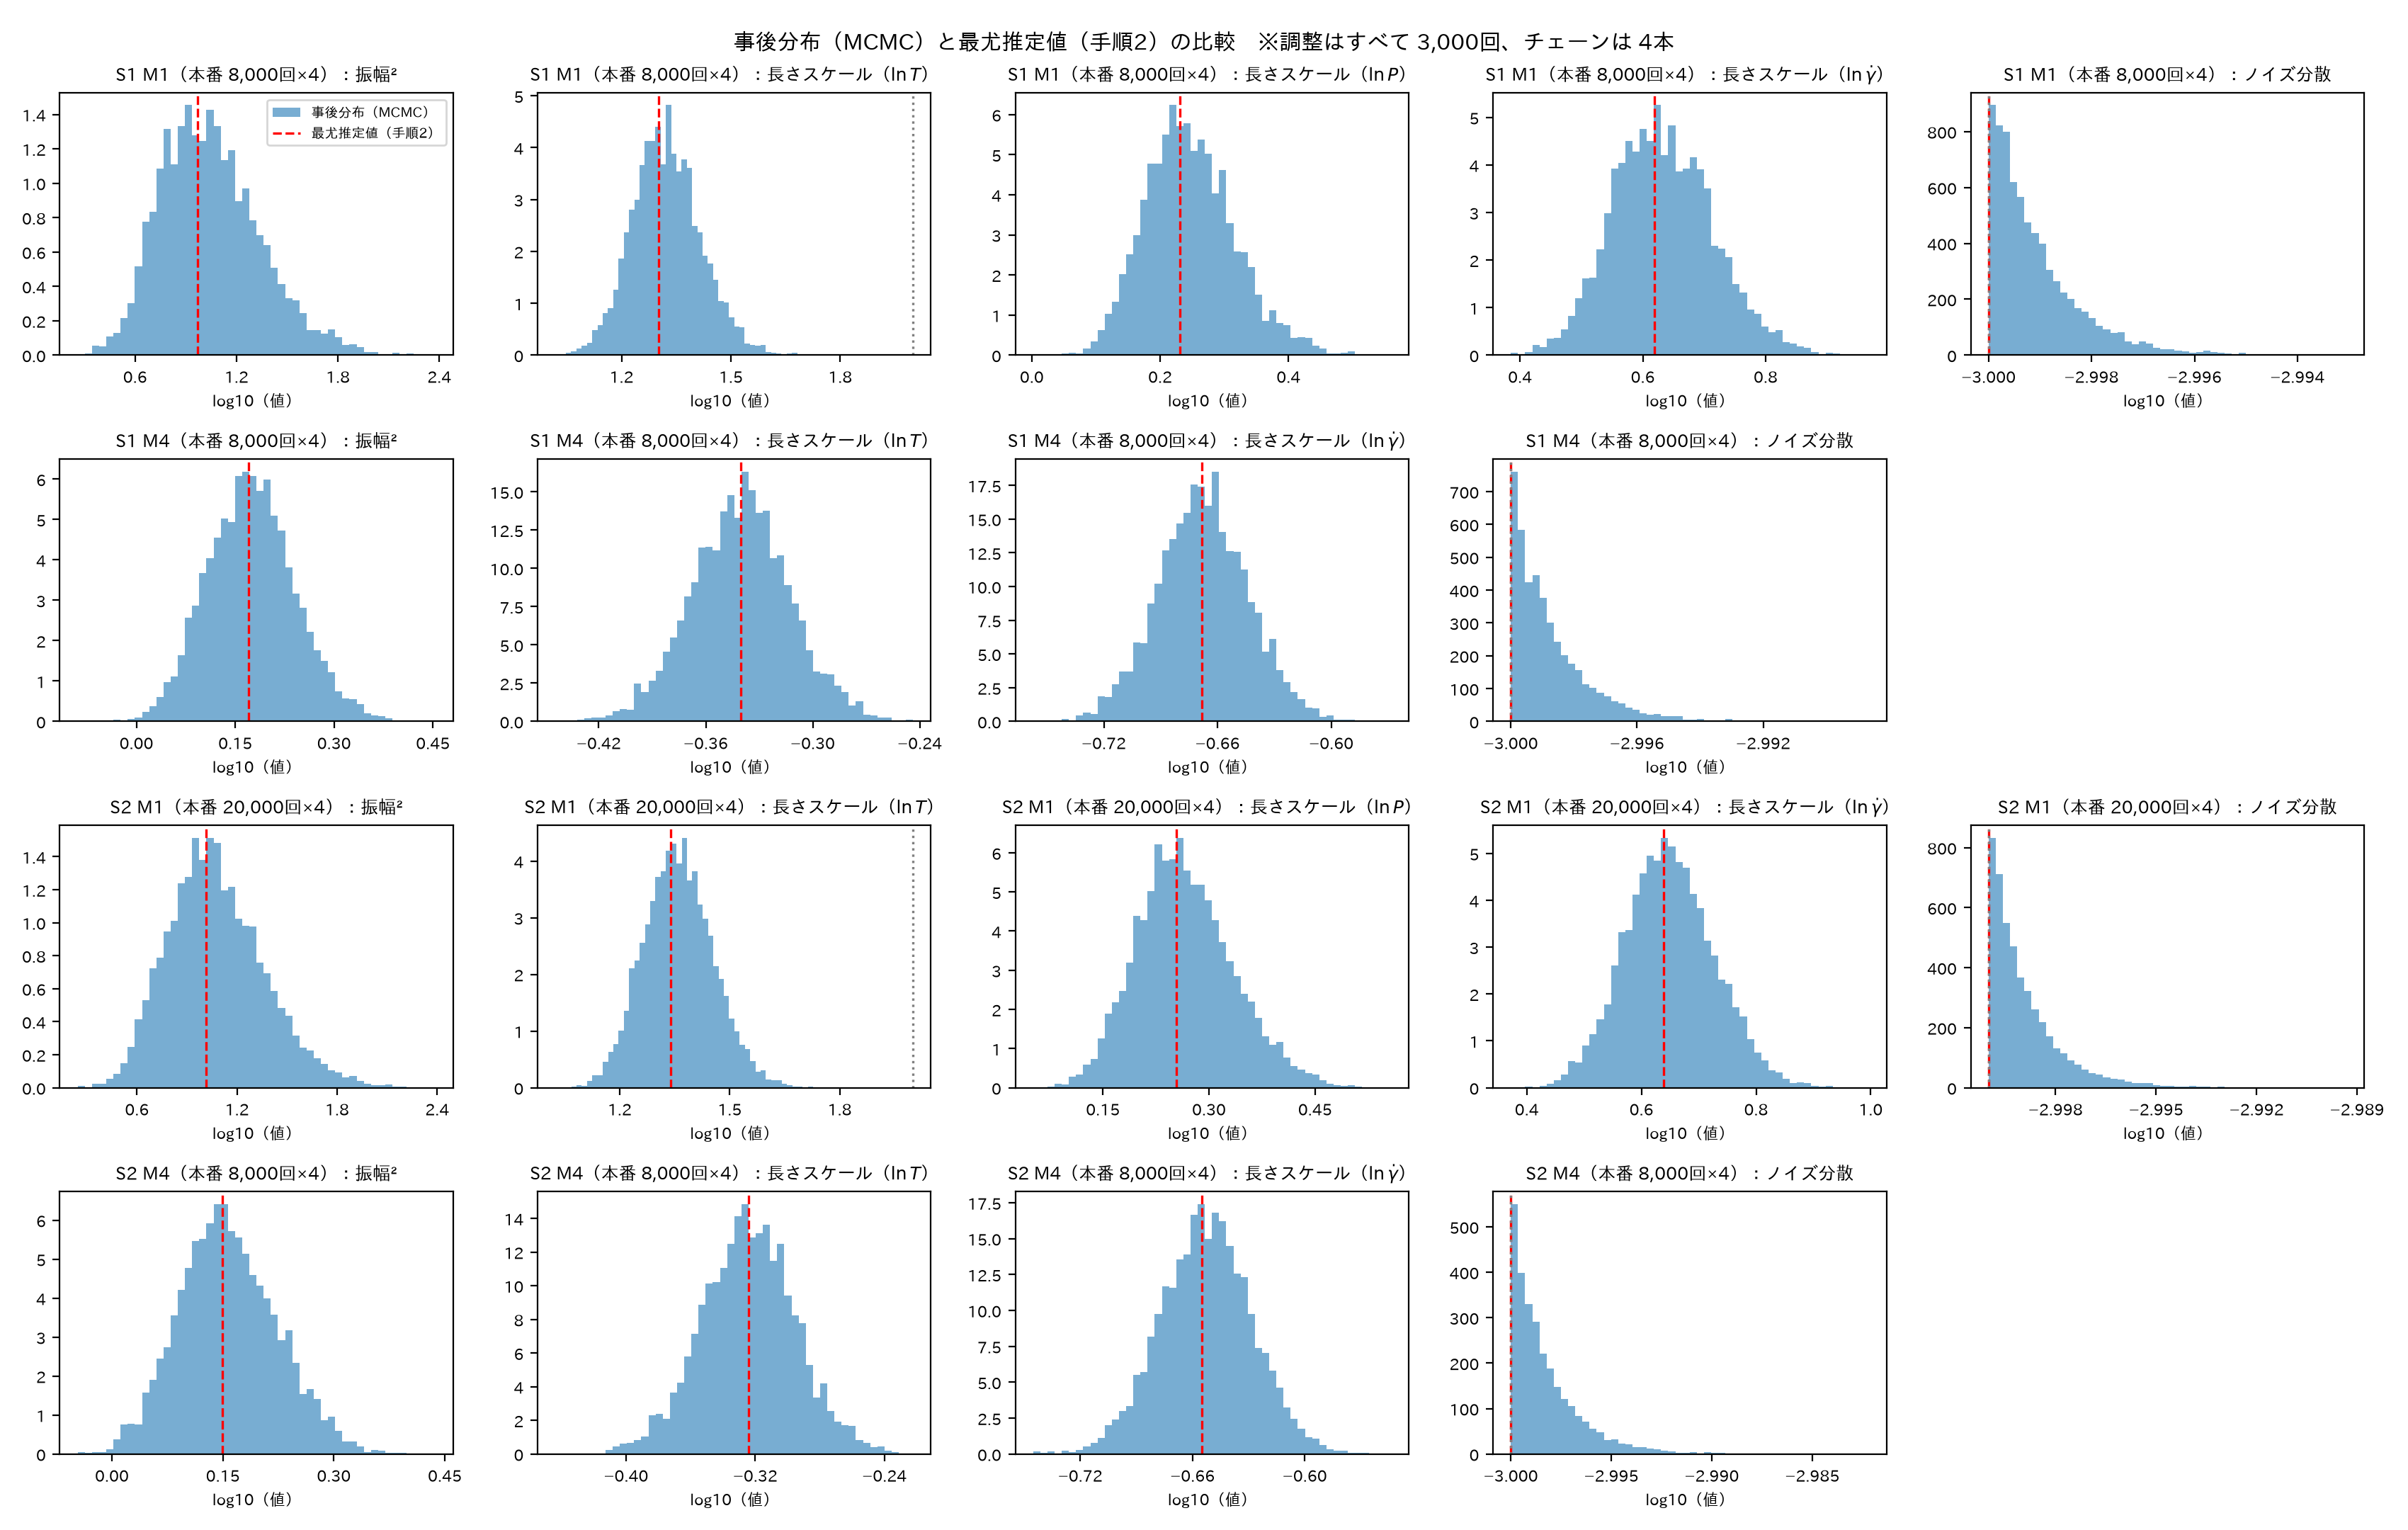
\includegraphics[width=\linewidth]{fig_posterior_vs_mle.png}
\caption{ハイパーパラメータの事後分布（青）と最尤推定値（赤の破線）}
\end{figure}
\begin{points}
\pt{ファイル}\file{results/step2_mcmc/fig_posterior_vs_mle.png}
\pt{何を示す図か}MCMC で求めたハイパーパラメータの事後分布（青のヒストグラム）と、手順2の最尤推定値（赤の破線）を比べる図です。行が組み合わせ、列がハイパーパラメータです。灰色の点線は探索範囲の端で、分布の近くにあるときだけ表示しています。
\pt{軸}横軸は値の $\log_{10}$、縦軸は割合（密度）です。
\pt{見るポイント}赤い破線が青い山のどこにあるか（山の中なら、最尤推定の値はもっともらしい値の一つ）。山の幅（広いほど、その値はデータから決まりにくく、不確か）。山が探索範囲の端で切れていないか。
\pt{今回の結果}赤い破線は、どれも青い山の中にあります。いちばん不確かなのは振幅で、S1・M1 の 95\% 信用区間は 1.90〜7.13 と幅があります（表）。$P$ の長さスケールが最も短く、$P$ が最もよく効いていることは、不確かさを考えても変わりません。ノイズ分散は下限の 0.001 で切れており、データはもっと小さいノイズを望んでいます。M4 の長さスケールは約 0.46（$T$）と 0.21（$\gd$）と短く、条件ごとの値を細かくなぞっていることを表しています。
\end{points}

\begin{table}[H]
\caption{S1・M1 のハイパーパラメータ（\file{step2_mcmc/posterior_summary.csv}。長さスケールは標準化後の入力に対する値）}
\begin{tabularx}{\linewidth}{@{}X*{3}{r}@{}}
\toprule
ハイパーパラメータ & 最尤推定値（手順2） & 事後分布の中央値 & 95\% 信用区間 \\
\midrule
振幅 & 3.05 & 3.24 & 1.90〜7.13 \\
長さスケール（$\ln T$） & 20.0 & 20.9 & 14.0〜32.9 \\
長さスケール（$\ln P$） & 1.70 & 1.74 & 1.33〜2.52 \\
長さスケール（$\ln\dot{\gamma}$） & 4.15 & 4.25 & 3.05〜6.34 \\
ノイズ分散 & 0.001000 & 0.001002 & 0.001000〜0.001007 \\
\bottomrule
\end{tabularx}
\end{table}

% ---------------------------------------------------------------------
\subsection{図10：パリティ図・MCMC 版}
\begin{figure}[H]
\centering
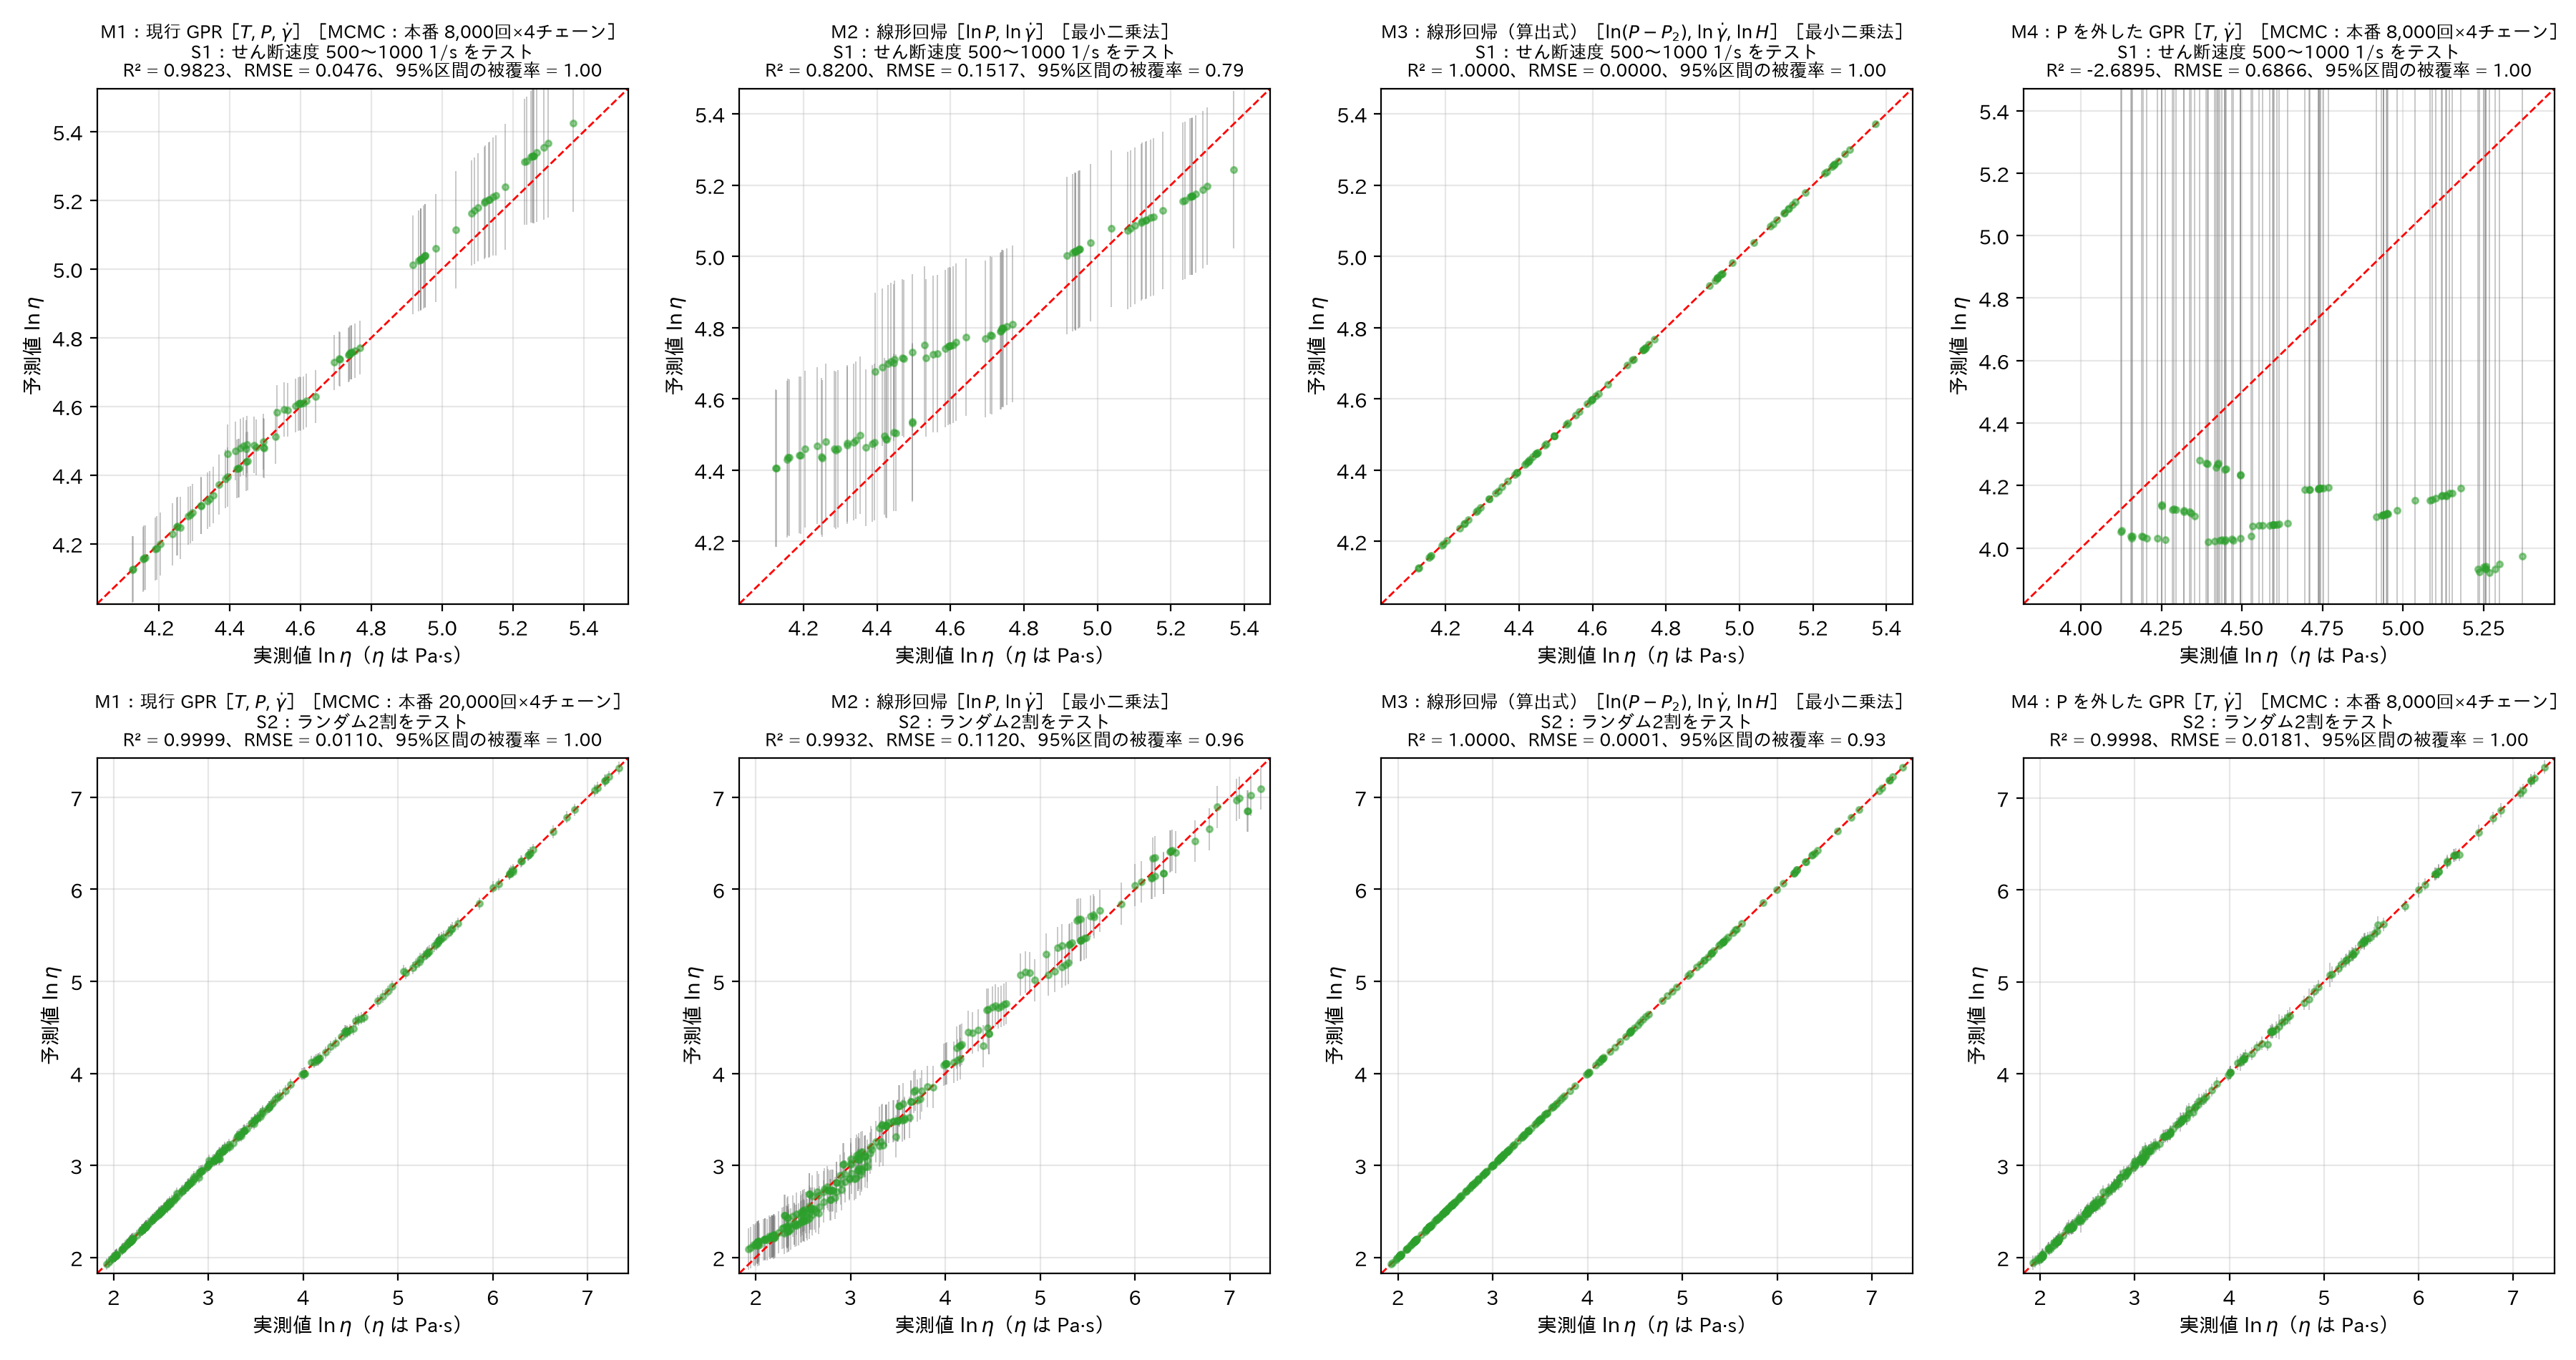
\includegraphics[width=\linewidth]{fig_parity_ln_eta_mcmc.png}
\caption{MCMC 版のパリティ図（M1・M4 は MCMC、M2・M3 は手順2と同じ）}
\end{figure}
\begin{points}
\pt{ファイル}\file{results/step2_mcmc/fig_parity_ln_eta_mcmc.png}
\pt{見方}図2と同じです。M1・M4 は MCMC の混合予測分布で予測し、M2・M3 は手順2と同じ線形回帰です。各パネルのタイトルに、MCMC の本番の回数を示しました。
\pt{今回の結果}手順2（最尤推定）とほとんど同じ結果になりました（表）。予測のばらつき（予測標準偏差の平均）は、MCMC のほうが 0〜3\% 大きくなっただけです。データが 1,000 行以上あるので、ハイパーパラメータの不確かさが予測に与える影響は小さく、1組の値（最尤推定）でもほぼ同じ予測になります。
\end{points}

\begin{table}[H]
\caption{MCMC と最尤推定の比較（\file{step2_mcmc/metrics.csv}。$\ln\eta$ で計算）}
\begin{tabularx}{\linewidth}{@{}X*{6}{r}@{}}
\toprule
 & \multicolumn{2}{c}{$R^2$} & \multicolumn{2}{c}{NLPD} & \multicolumn{2}{c}{予測標準偏差の平均} \\
\cmidrule(lr){2-3}\cmidrule(lr){4-5}\cmidrule(l){6-7}
組み合わせ & MCMC & 最尤推定 & MCMC & 最尤推定 & MCMC & 最尤推定 \\
\midrule
S1・M1 & 0.9823 & 0.9823 & $-1.779$ & $-1.781$ & 0.0581 & 0.0565 \\
S1・M4 & $-2.6895$ & $-2.6793$ & 1.177 & 1.173 & 1.0626 & 1.0548 \\
S2・M1 & 0.9999 & 0.9999 & $-2.438$ & $-2.439$ & 0.0330 & 0.0329 \\
S2・M4 & 0.9998 & 0.9998 & $-2.277$ & $-2.279$ & 0.0364 & 0.0363 \\
\bottomrule
\end{tabularx}
\end{table}

% ---------------------------------------------------------------------
\subsection{図11：M1 の予測曲線・MCMC 版}
\begin{figure}[H]
\centering
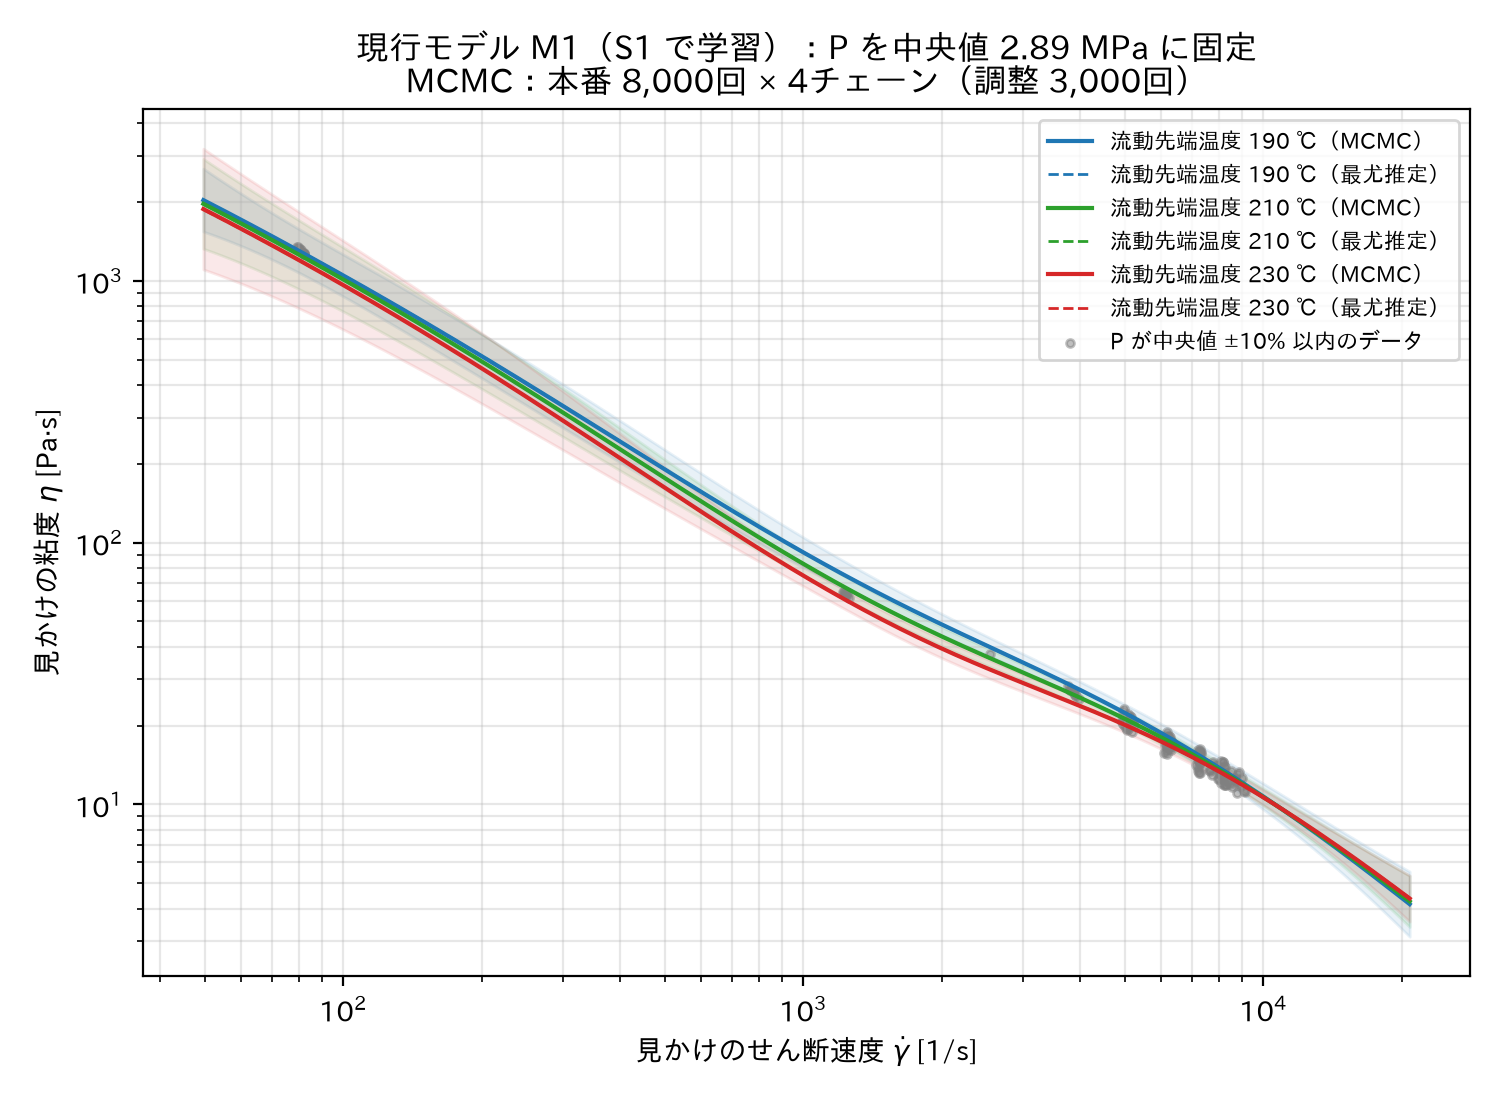
\includegraphics[width=0.74\linewidth]{fig_M1_curves_by_T_mcmc.png}
\caption{MCMC 版の M1 の予測曲線（実線と帯は MCMC、破線は最尤推定）}
\end{figure}
\begin{points}
\pt{ファイル}\file{results/step2_mcmc/fig_M1_curves_by_T_mcmc.png}
\pt{見方}図4と同じです。実線と帯が MCMC、破線が最尤推定です。タイトルに MCMC の本番の回数を示しました。
\pt{今回の結果}MCMC と最尤推定の曲線は重なり、見分けがつきません。傾きは約 $-0.99$、190 ℃ と 230 ℃ の差は最大 1.24 倍で、図4と同じです。ハイパーパラメータの決め方を変えても、「$P$ を固定すると温度の効果が表に出ない」という結論は変わりません。
\end{points}

% =====================================================================
\section{表（CSV）の見方}

各フォルダの CSV ファイルの中身と、主な列の意味です。$\ln$ は自然対数です。

\begin{table}[H]
\caption{\file{results/step2/} の表}
\begin{tabularx}{\linewidth}{@{}>{\raggedright\arraybackslash}p{13\zw}X@{}}
\toprule
ファイル & 中身と主な列 \\
\midrule
\file{metrics.csv} & 分け方・モデルごとのテストの指標。\file{R2_ln_eta}（$\ln\eta$ の $R^2$）、\file{RMSE_ln_eta}、\file{R2_eta}（粘度そのものの $R^2$）、\file{coverage95}（被覆率）、\file{NLPD}。 \\
\file{kernels.csv} & GPR のハイパーパラメータの最尤推定値。\file{amplitude}（振幅）、\file{ls_lnT}・\file{ls_lnP}・\file{ls_lnSR}（長さスケール）、\file{noise_level}（ノイズ分散）、\file{LML}（対数周辺尤度）、\file{fit_seconds}（学習時間）。 \\
\file{ols_coefficients.csv} & 線形回帰（M2・M3）の係数。\file{intercept}（定数）、\file{b_*}（各入力の係数）、\file{resid_sd}（残差の標準偏差）。 \\
\file{formula_check.csv} & 粘度の算出式の確認（図1）。\file{L_mm}（センサ間距離）、\file{P2_MPa}、\file{max_abs_rel_resid_pct}（式からのずれの最大値、\%）。 \\
\file{temperature_effect_}\newline\file{190_vs_230.csv} & 同じ厚み・射出率での 190 ℃ と 230 ℃ の比較（図3）。\file{ln_eta}・\file{ln_sr} は $\ln$ の差で、exp をとると比になる。 \\
\bottomrule
\end{tabularx}
\end{table}

\begin{table}[H]
\caption{\file{results/step2_mcmc/} の表}
\begin{tabularx}{\linewidth}{@{}>{\raggedright\arraybackslash}p{13\zw}X@{}}
\toprule
ファイル & 中身と主な列 \\
\midrule
\file{metrics.csv} & テストの指標。\file{method} は MCMC・MLE（最尤推定）・OLS（線形回帰）。MCMC の行には、\file{chains}（チェーン数）、\file{n_warm}（調整の回数）、\file{n_samp_per_chain}（1チェーンの本番の回数）、\file{draws_total}（本番のサンプルの合計）も入っている。\file{mean_pred_sd} は予測標準偏差の平均。 \\
\file{posterior_summary.csv} & ハイパーパラメータの事後分布の要約。\file{MLE}（最尤推定値）、\file{post_mean}・\file{post_sd}（平均・標準偏差）、\file{q2.5}・\file{median}・\file{q97.5}（2.5\% 点・中央値・97.5\% 点）、\file{r_hat}、\file{ess_bulk}・\file{ess_tail}。 \\
\file{sampler_stats.csv} & 組み合わせごとのサンプリングの回数と収束。採択率の最小・最大、\file{sampling_min}（時間、分）、\file{max_r_hat}、\file{min_ess_bulk}・\file{min_ess_tail}。 \\
\file{chain_info.csv} & チェーンごとの採択率（\file{acc_warm}：調整、\file{acc_samp}：本番）、提案の大きさ \file{lambda}、時間。 \\
\file{posterior_S1_M1.csv} など & 本番のサンプルすべて。\file{chain}、\file{draw}、\file{log_c}（$\ln$ 振幅$^2$）、\file{log_ls_*}（$\ln$ 長さスケール）、\file{log_noise}（$\ln$ ノイズ分散）、\file{lp}（対数事後密度）、\file{accepted}（候補を受け入れたら 1）。 \\
\bottomrule
\end{tabularx}
\end{table}

% =====================================================================
\section{結果のまとめ}

\begin{enumerate}[itemsep=0.6ex,topsep=0.6ex]
\item \textbf{リーク}：粘度は $P$・$\gd$・厚みから計算されています（図1）。$P$ を入力にした現行モデルの高い精度は、この計算式を覚えたことによるものです。$P$ を外すと、S1 ではまったく予測できません（図2、$R^2$ = $-2.68$）。
\item \textbf{評価の甘さ}：ランダムな分け方（S2）では、同じ条件のショットが学習データにも入るので、$P$ を外しても精度が高く見えます（$R^2$ = 0.9998）。評価は、条件単位の分け方で行う必要があります。
\item \textbf{温度の効果}：データには温度の効果がはっきりあります（190 ℃ の粘度は 230 ℃ の約 1.24 倍、図3）。しかし現行モデルでは $P$ に吸収されて、表に出てきません（図4）。
\item \textbf{MCMC}：ハイパーパラメータを MCMC で推定しても、予測はほとんど変わらず（予測のばらつきが 0〜3\% 広がる程度）、上の結論も変わりません（図9〜11）。
\item \textbf{次の手順}：条件単位の分け方を作り（手順3）、$P$ と流動先端温度を使わない新しいモデル（設定温度・せん断速度・厚みを使う）を作って評価します（手順4・5）。
\end{enumerate}

\end{document}
